\chapter{Introduction}
% \section{1.1}
% \subsection{1.1.1}



% Absatze werden in Latex durch eine Leerzeile voneinder getrennt. Die Grundlagen zur UML/P finden sich in \cite{Rum11}

% Anstatt die Absatze durch einen grosseren Abstand voneinander zu trennen, kann man auch die erste Zeile einrucken.

% Eine Website zitiert man so \cite{SE10} und hier gibt es MontiCore \cite{Mon10}. 

% Das sieht dann z.B. so aus ...
% \setlength{\parindent}{3ex}
% \setlength{\parskip}{0ex}

% Neuer Absatz ... Neuer Absatz ... Neuer Absatz ... Neuer Absatz ... Neuer Absatz ... Neuer Absatz ... Neuer Absatz ... Neuer Absatz ...

% Neuer Absatz ... Neuer Absatz ... Neuer Absatz ... Neuer Absatz ... Neuer Absatz ... Neuer Absatz ... Neuer Absatz ... Neuer Absatz ...

% Eine der beiden Varianten MUSS man wahlen, welche ist jedoch egal.

\section{What is HIS?}
Hospital information systems (HIS) have become a fundamental component of modern healthcare organizations, enabling efficient patient data management, improving clinical decision-making, and enhancing healthcare delivery. \cite{HIS} A HIS is a socio-technical system consisting not only of components like software or hardware but also integrates the human aspect of staff working with these components or patients. The effective modeling of hospital information systems is crucial to ensure their successful implementation and operation, as it facilitates decision-making processes, enhances system performance, and supports the seamless integration of various components.

\section{Motivation:}
The motivation behind this research paper stems from the increasing reliance on information technology in the healthcare sector and the need for robust and well-designed hospital information systems. As healthcare organizations strive to deliver high-quality care while managing vast amounts of patient data, it is essential to understand and apply modeling techniques to develop efficient and effective HIS.

Despite the growing importance of hospital information systems, a research gap exists regarding the modeling approaches and methodologies tailored explicitly to these systems. While general software engineering principles and modeling techniques have been widely applied in other domains, hospital information systems' unique characteristics and complexities necessitate specialized modeling methods. This paper addresses this research gap by comprehensively analyzing the modeling techniques used in HIS design and implementation.

\section{Objectives:}

The primary objective of this research paper is to provide a comprehensive overview of the modeling techniques employed in hospital information systems. By focusing on modeling approaches such as class diagrams, use case diagrams, BPMN diagrams, and sequence diagrams, this paper aims to present a range of models that capture different aspects of HIS functionality and behavior. Through this analysis, the paper seeks to enhance the understanding of stakeholders, including healthcare administrators, IT professionals, and researchers, and provide them with valuable insights to make informed decisions during the design and implementation phases of HIS.

This research paper holds significant implications for both academia and industry. For academia, it contributes to the body of knowledge in the field of healthcare informatics by shedding light on the modeling techniques specifically relevant to hospital information systems. Exploring various models, such as class diagrams, use case diagrams, BPMN diagrams, and sequence diagrams, in the context of HIS will aid researchers in developing more accurate and effective modeling approaches.

In the industry, this paper serves as a practical guide for healthcare administrators and IT professionals involved in designing, developing, and implementing hospital information systems. By providing insights into different modeling techniques, it empowers stakeholders to make informed decisions during the system's lifecycle, ensuring that the resulting HIS meets the specific needs and requirements of the healthcare organization. Moreover, the presented models serve as a reference for practitioners, enabling them to adopt best practices and enhance their systems' overall quality and efficiency.

% \section{Structure of the Paper: Not sure}

% The remainder of this paper is organized as follows. Section 2 provides an overview of the key components of hospital information systems, highlighting the interconnected nature of these components and their role in supporting healthcare organizations. Section 3 presents an in-depth analysis of the modeling approaches and methodologies employed in the design of HIS, with a focus on class diagrams, use case diagrams, BPMN diagrams, and sequence diagrams. Section 4 discusses the challenges and considerations associated with modeling hospital information systems, including privacy and security, scalability and performance, and user acceptance and adoption. Finally, Section 5 concludes the paper by summarizing the key findings, discussing potential future research directions, and emphasizing the importance of effective modeling in advancing hospital information systems.



\cleardoublepage



\chapter{Background}
\section{Domain Background}
The domain of hospital information systems revolves around managing and utilizing patient data within healthcare organizations. With the advancement of technology, hospitals have transitioned from paper-based record-keeping systems to electronic systems that streamline patient information collection, storage, and retrieval. Hospital information systems encompass various components, including electronic health records, clinical decision support systems, computerized physician order entry systems, and hospital billing and administrative systems. These systems are critical in improving patient care, optimizing workflows, and supporting informed decision-making by healthcare professionals. Figure 2.1 below explains the typical tasks in a Hospital.

\begin{figure}[ht!]
\begin{center}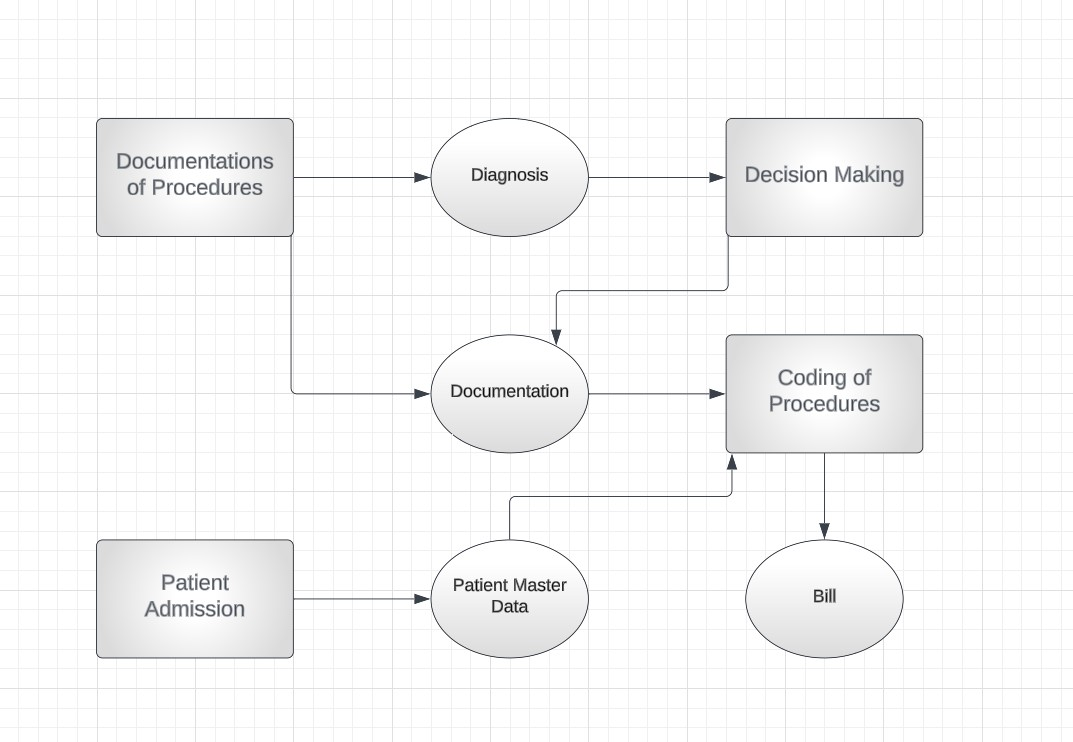
\includegraphics[width=12cm]{src/pic/Typical_Medical_Procedure.jpg}\end{center}
\caption{Typical Medical Structure \cite{Ben20}}
\label{TMP}
\end{figure}


\section{Modeling Concepts}
To effectively design and represent hospital information systems, this paper utilizes modeling concepts such as Monticore and Business Process Model and Notation (BPMN), which are explained a bit further in more detail.

\subsection{Monticore}

Monticore is a domain-specific modeling language and toolset that provides support for modeling, analysis, and code generation. It is widely used in software engineering and system design to create models that capture the structure, behavior, and interactions of complex systems. Monticore facilitates the creation of models using various diagrammatic notations and allows for the specification of model constraints, transformations, and code generation. \cite{Monticore:Framework}

In the context of this paper, Monticore is utilized to create models such as class diagrams, use case diagrams, and sequence diagrams to represent different aspects of hospital information systems. Class diagrams help visualize the structure and relationships between the various entities and data elements within the system. Use case diagrams capture the functionalities and interactions between system users and the system itself. Sequence diagrams illustrate the dynamic behavior and flow of activities within the system, particularly during specific processes or scenarios. 

By utilizing Monticore, this paper leverages a powerful modeling language and toolset to effectively represent and analyze the various components and functionalities of hospital information systems.

Below we will summarize the languages from the Monticore Catalog that we used for modelling various aspects of Hospital Information Systems - 

\subsubsection{Class Diagram For Analysis (CD4A)}
CD4A is a concise textual representation of UML class diagrams, explicitly utilizing the UML/P variant (“P” in UML/P stands for “suitable for programming”). It covers the essential elements of class diagrams, including classes, interfaces, inheritance, attributes with types and visibilities, and various association and composition types, such as qualified and ordered associations. CD4A allows software engineers to represent complex class structures and accurately depict relationships between classes while maintaining code reusability and modularity through inheritance. Including attributes with associated types and visibilities ensures a comprehensive representation of class characteristics. CD4A is a compact, human-readable alternative to graphical UML tools, facilitating collaboration, version control, and documentation.\cite{MontiCore}
 
 
\subsubsection{Sequence Diagrams (SD)}
SD is a textual language that allows for the representation of sequence diagrams (SDs). The project encompasses grammar, a symbol table infrastructure, a PrettyPrinter, and several CoCos for type-checking. The language is divided into two grammars: SDBasis and SD4Development. SDBasis serves as a foundational grammar, providing essential features of the SD language.\cite{MontiCore}


\subsubsection{Use Case Diagrams (UCD)}

UCD is a textual language designed to represent use case diagrams (UCDs). The project comprises a grammar, a symbol table infrastructure, and a semantic differencing operator. The language is defined by the UCD grammar, which provides the necessary syntax and rules to describe use case diagrams.

UCD allows for modelling various elements, including actors, use cases, preconditions, associations between actors and use cases, extend relations between use cases with guards, including relations between use cases, and specialization relations between actors and use cases. These elements capture the interactions and relationships between actors and use cases in a system, visually representing the system's functional requirements.\cite{MontiCore}


\subsection{Business Process Model and Notation (BPMN)}


BPMN is a standardized graphical notation for modeling business processes. It visually represents business workflows, activities, decisions, and the flow of data or information within an organization. BPMN diagrams offer a clear and intuitive way to depict the sequence of activities, decision points, and the involvement of different stakeholders in a process. \footnote{BPMN Website 
\url{https://www.bpmn.org/}.}

In hospital information systems, BPMN diagrams are valuable for modeling and analyzing the workflows and processes involved in patient care, administrative tasks, and other activities within the healthcare organization. BPMN diagrams help stakeholders understand the sequence of activities, identify bottlenecks, and improve the efficiency of processes. 

By utilizing BPMN in this paper, we can effectively represent the complex workflows and interactions within hospital information systems, contributing to a better understanding of the system's behavior and facilitating process optimization. \cite{Aagesen2015}



\begin{figure}[!htb]
\begin{center}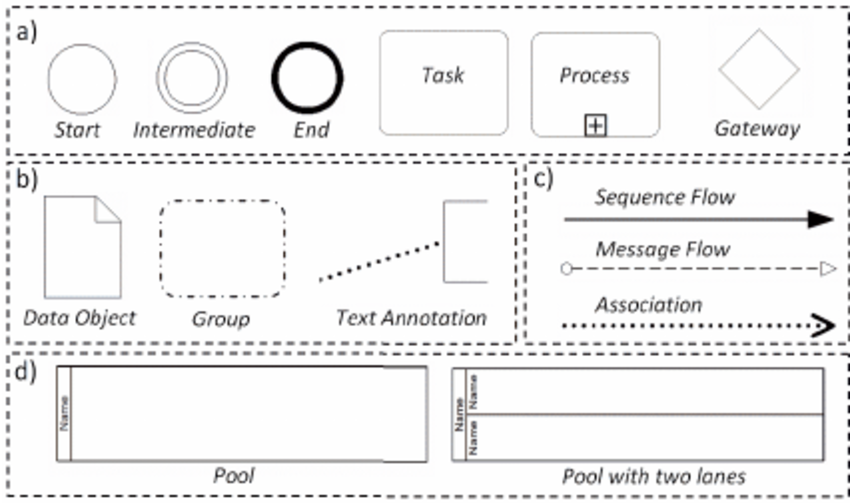
\includegraphics[width=12cm]{src/pic/Basic_BPMN.png}\end{center}
\caption{Basic Elements of BPMN 2.0 \cite{BPMN_Basic}}
\label{BBPMN}
\end{figure}


\let\cleardoublepage\clearpage